\begin{center}
  \Large
  \textbf{BIOGRAFI PENULIS}
\end{center}

\addcontentsline{toc}{chapter}{BIOGRAFI PENULIS}

\vspace{2ex}

\begin{wrapfigure}{L}{0.3\textwidth}
  \centering
  \vspace{-3ex}
  % Ubah file gambar berikut dengan file foto dari mahasiswa
  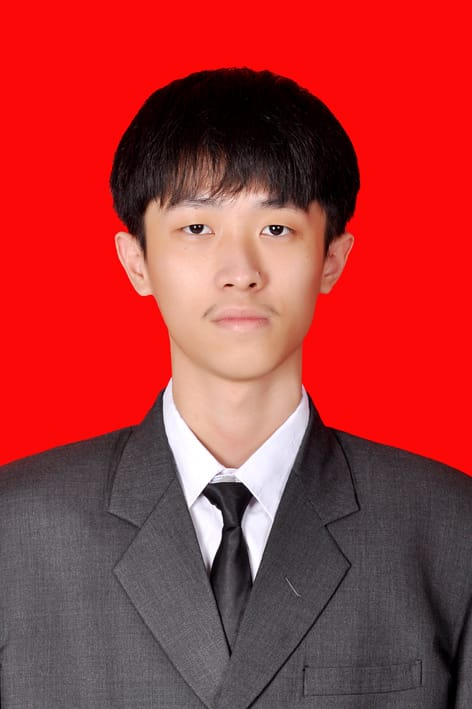
\includegraphics[width=0.3\textwidth]{gambar/nathan.jpg}
  \vspace{-4ex}
\end{wrapfigure}

Penulis bernama \name{} yang akrab disapa Nathan, lahir pada tanggal 24 August 2001 di kota Surabaya, Jawa Timur.
Penulis telah menempuh pendidikan di SD Katolik Sang Timur Pasuruan lulus pada tahun 2013, SMP Katolik Sang Timur Pasuruan lulus pada tahun 2016, dan SMA Katolik St. Louis 1 Surabaya lulus pada tahun 2019.
Penulis kemudian melanjutkan pendidikan sarjana di Departemen Teknik Komputer Institut Teknologi Sepuluh Nopember melalui jalur SBMPTN pada tahun 2019.
Selama aktif menjadi mahasiswa, penulis telah bergabung ke dalam dalam Tim Robotika Ichiro sebagai \textit{programmer} dan Asisten Laboratorium B401.
Sebagai bagian dari Tim Ichiro, penulis telah meraih beberapa prestasi nasional dan internasional seperti Kontes Robot Indonesia Nasional 2020 dan 2021, FIRA SimulCup 2021 dan 2022 yang diselenggarakan secara daring,
serta Kontes Robot Indonesia Nasional 2022 dan RoboCup 2022 Bangkok yang diselenggarakan secara luring
Penulis juga telah bergabung dengan Bangkit Academy 2022 pada jalur \textit{Machine Learning} dan memiliki pengalaman magang selama 3 bulan di PT Indosat Tbk untuk menyelesaikan Program Bangkit Academy.
Minat penulis dalam mengerjakan tugas akhir adalah \textit{Machine Learning} dan \textit{Computer Vision}. Penulis dapat dihubungi melalui email nathanael.hutama24@gmail.com.